\section{Evaluation}
\label{section_6}

%%%%%%%%%%%%%%%%%%%%%%%%%%%%%%%%%%%%%%%%%%%%%%%%%%
% \begin{table*}[t]
%         \centering
%         \caption{Zero-shot accuracy results on AIME 2025, Math-500, GPQA-Diamond}
%         \vspace{-1.0ex}
%         \includegraphics[width=1.0\linewidth]{Tables/7_1_Quantization_Accuracy_Comparison.pdf}
%         \label{6_2_accuracy_table}
%         \vspace{-1.0ex}
% \end{table*}
%%%%%%%%%%%%%%%%%%%%%%%%%%%%%%%%%%%%%%%%%%%%%%%%%%

%%%%%%%%%%%%%%%%%%%%%%%%%%%%%%%%%%%%%%%%%%%%%%%%%%
\begin{figure*}[t]
\centering
\footnotesize
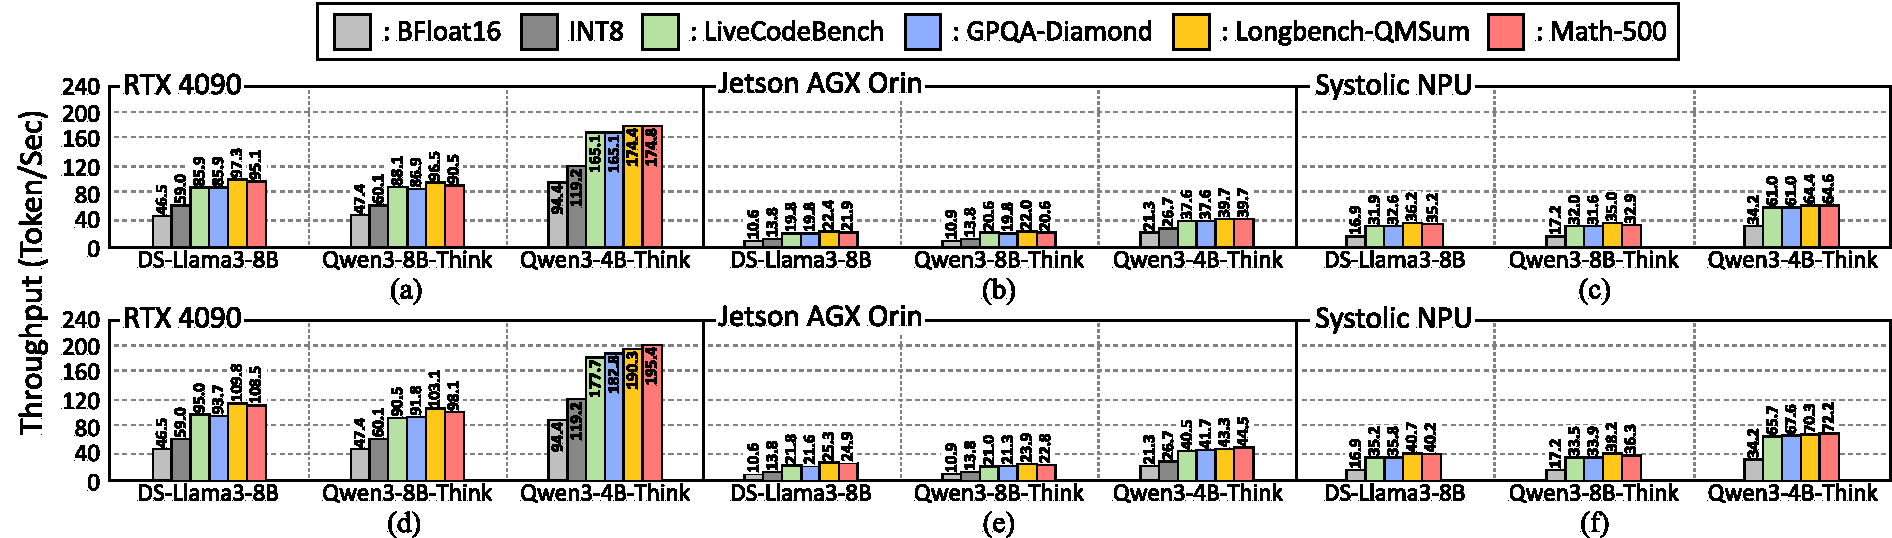
\includegraphics[width=\fullimgwidth]{Figures/6_3_Hardware_Performance.pdf}
\caption{Normalized performance gain through Cassandra on various hardware \& benchmark. (a) RTX 4090 + Cassandra-1, (b) Jetson AGX Orin + Cassandra-1, (c) Systolic Array NPU + Cassandra-1, (d) RTX 4090 + Cassandra-2, (e) Jetson AGX Orin + Cassandra-2, (f) Systolic Array NPU + Cassandra-2}
\label{fig_6_1} 
% \vspace{-1.5em}
\end{figure*}
%%%%%%%%%%%%%%%%%%%%%%%%%%%%%%%%%%%%%%%%%%%%%%%%%%%

\subsection{Implementation of Cassandra}
\label{section_6_1}
~\textbf{Cassandra Software Implementation.} To measure the accuracy of Cassandra, we developed a software emulator utilizing PyTorch and custom CUDA kernels. Although this software emulator cannot achieve performance gain on a GPU, it accurately models the pruning, truncation, unary coding, and MX format conversion that occur during the format transformation process in Cassandra.

~\textbf{Cassandra Hardware Implementation.} The performance of Cassandra cannot be characterized solely by hardware cycles; it also depends on the acceptance rate. Therefore, to measure the performance gain obtained by Cassandra, we first determine four different scenarios from benchmarks~\cite{LiveCodeBench, PRM800K(source_of_math_500), Longbench, GPQA-Diamond} and apply them to Cassandra with 40\% pruned and 4-bit truncated weights and 4-bit truncated KV cache. In addition, we measure the average input and output context lengths, as well as the acceptance rate for those scenarios. Finally, we use this information with the cycle information from our hardware simulator to quantify overall system performance.

To measure the performance of Cassandra when integrated with a GPU, we implement the Cassandra encoder and decoder on Accel-Sim~\cite{Accel-Sim}. We use Nvidia RTX 4090~\cite{RTX4090} and Nvidia Jetson AGX Orin~\cite{Jetson} as GPU baselines. Since Accel-Sim currently does not support the Ada-Lovelace architecture used in the RTX 4090, we use traces from an Ampere architecture GPU and set the configuration similar to RTX 4090.

Additionally, to evaluate the performance of Cassandra-integrated NPU, we implemented a cycle-level simulator by extending Scale-Sim~\cite{Scale-Sim} and the LPU simulator~\cite {LPU, oaken}. Referring to the specifications of commercial consumer-grade GPUs, we designed this NPU to feature a 64 TFLOPS MAC unit and a memory bandwidth of 273 GB/s, utilizing 128GB of LPDDR5X memory.

To analyze the power and area overhead of Cassandra, we first implement an end-to-end Cassandra decoder and encoder with SystemVerilog. We also implement a simple consumer-grade NPU, consisting of a systolic array, VPU, DMA, and scratchpad, and integrate it with Cassandra. Both Cassandra and NPU are synthesized using the Synopsys Design Compiler with a 28nm technology node, and the area of the SRAM used was obtained by utilizing the Samsung 28nm SRAM Compiler.
% Also, to ensure a fair comparison with the GPU, we scale Cassandra's power and area to the same process technology as the target GPU with DeepScaleTool~\cite{DeepScaleTool}.



%%%%%%%%%%%%%%%%%%%%%%%%%%%%%%%%%%%%%%%%%%%%%%%%%%%%%%%%%%%%
\begin{table}[t]
\caption{Zero-shot accuracy results on Reasoning Benchmarks}
\centering
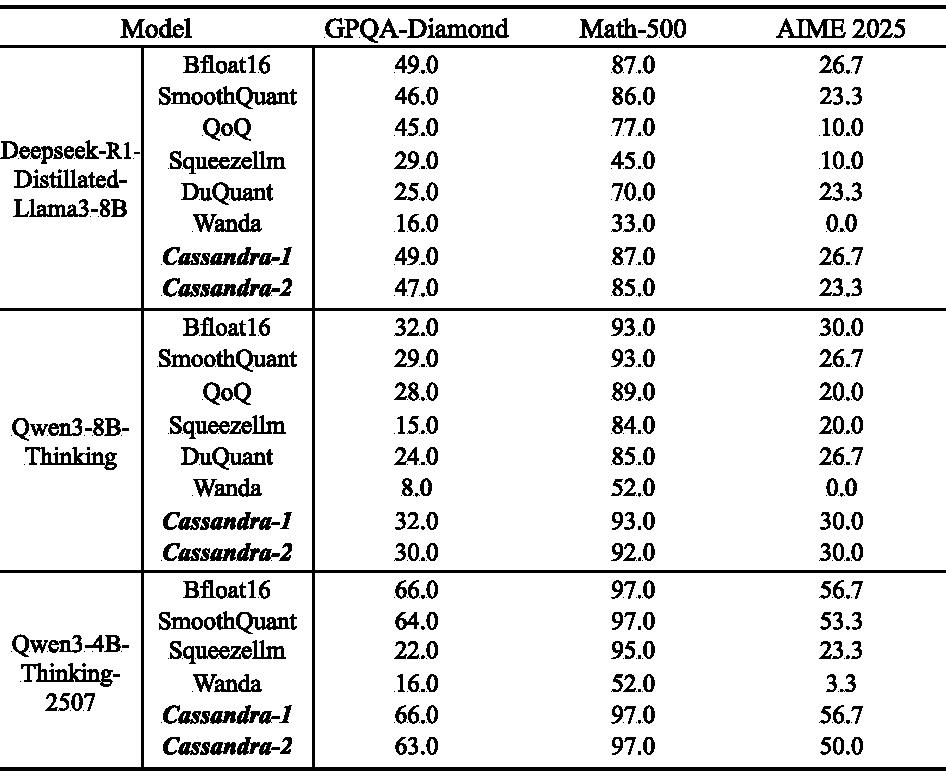
\includegraphics[width=\colimgwidth]{Tables/6_1_Quantization_Accuracy_New.pdf}
\label{6_2_accuracy_table}
\vspace{-3.0em}
\end{table}
%%%%%%%%%%%%%%%%%%%%%%%%%%%%%%%%%%%%%%%%%%%%%%%%%%%%%%%%%%%%

\subsection{Zero-Shot Accuracy Evaluation}
\label{section_6_2}

In this part, we compare state-of-the-art lossy compression methods~\cite{Smoothquant, qserve, duquant, Wanda, squeezellm} with Cassandra across various benchmarks. The pruning ratio and precision used for lossy compression are identical to those in the original papers. We use Deepseek-R1-Distillated-Llama3-8B~\cite{Deepseek-R1-Distillated-Llama3-8B}, Qwen3-8B-Thinking~\cite{Qwen3-8B}, and Qwen3-4B-Thinking-2507~\cite{Qwen3-4B-Thinking-2507} as LLM models and use AIME2025~\cite{AIME2025}, Math-500~\cite{PRM800K(source_of_math_500)}, GPQA-Diamond~\cite{GPQA-Diamond} as benchmarks. Due to the limited GPU resources, we randomly sampled 100 questions from the GPQA-Diamond and Math-500, while the AIME2025 benchmark was tested using all its questions. Table~\ref{6_2_accuracy_table} compares Cassandra with other lossy compression techniques with these models and benchmarks. 

As illustrated in the table, all lossy compression methods experience a certain degree of accuracy degradation. Smoothquant, which utilizes relatively higher bitwidth, exhibits only a marginal drop in accuracy compared to the BFloat16 baseline; however, its compression ratio remains modest at approximately 50\%.
In contrast, all other lossy compression techniques suffered significant accuracy losses across reasoning benchmarks. Notably, when applied to DeepSeek-R1-Distillated-Llama3-8B, Wanda failed to produce a single correct answer on the AIME 2025 benchmark.
Conversely, Cassandra-1 maintained accuracy levels identical to BFloat16. Also, Cassandra-2, which prioritizes inference speed at the expense of some precision, demonstrated a robust accuracy profile comparable to that of Smoothquant.

% Furthermore, as seen in the table, DuQuant~\cite{duquant} and QoQ~\cite{qserve} were not applied to the Qwen3-4B model. This is because these methods apply a matrix rotation based on the Hadamard transformation to minimize accuracy loss caused by outliers. While rotation is one of the key methods in modern LLM quantization~\cite{QuaRot, SpinQuant}, it cannot be applied to LLMs that have hidden dimension sizes mathematically incompatible with the Hadamard matrix~\cite{Qwen3-4B}. This limitation in usability is also one of the drawbacks of state-of-the-art low-bit quantization, and the relatively broad scalability across various models is also one of the strengths of Cassandra.

As illustrated in the table, DuQuant~\cite{duquant} and QoQ~\cite{qserve} were not evaluated on the Qwen3-4B-Thinking-2507 model. These algorithms maintain model accuracy by employing Hadamard rotations to smooth out the distribution of values, thereby reducing the impact of outliers. However, since Hadamard matrices are restricted to specific discrete dimensions, their open-source implementations are not directly compatible with the unique hidden dimension of Qwen3-4B-Thinking-2507. Applying these methods would require additional pre-processing, such as zero padding.

\subsection{Performance}
\label{section_6_3}
Figure~\ref{fig_6_1} presents Cassandra's overall performance gain obtained from our simulator. Since Cassandra's performance varies depending on the model and the benchmark, we express its performance using the throughput gain achievable across four different scenarios, three models, and various exponent compression techniques. Furthermore, the length of the draft tokens $\gamma$ is set to the value that yielded optimal performance within the range of 3 to 5.
Furthermore, we included SmoothQuant-based W8A8 integer quantization~\cite{Smoothquant} as a GPU baseline, utilizing the official INT8 quantization implementation provided by vLLM~\cite{W8A8-INT8-Dynamic}. While we also measured the throughput of FP8 dynamic quantization~\cite{W8A8-FP8-Dynamic} on an RTX 4090, it consistently showed a slight performance deficit in the decode stage compared to INT8. However, this performance gap was marginal, staying under 3\% for all tested models.


\begin{table}[t]
\caption{Average Acceptance Rate on Various Models and Benchmarks.}
\centering
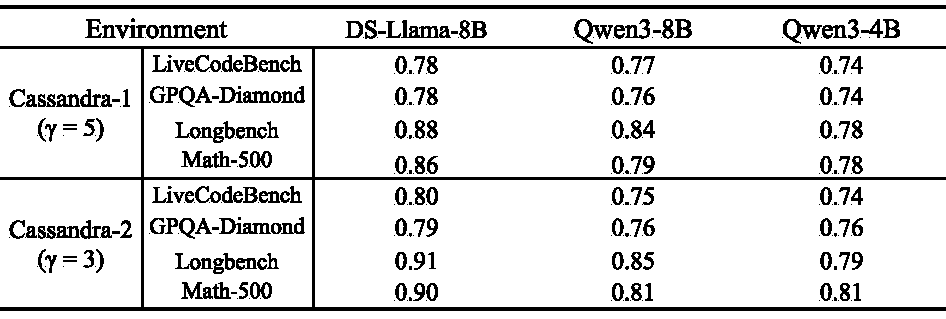
\includegraphics[width=\colimgwidth]{Tables/6_3_average_acceptance_rate.pdf}
\label{table_6_3}
\vspace{-0.20in}
\end{table}

As shown in the figure, Cassandra achieved a performance improvement of 1.78$\times$ to 2.41$\times$ compared to BFloat16 baseline. Two primary factors influence the performance of Cassandra. One factor is the disparity between models. As shown in Table~\ref{table_6_3}, under identical configurations and benchmarks, DeepSeek-R1-Distillated-Llama3-8B typically exhibited the highest acceptance rate, followed by Qwen3-8B and Qwen3-4B-Thinking-2507, respectively. The second factor is the difference of benchmark. Across all models, Cassandra performed slightly better on Longbench-QMSum and Math500 than on LiveCodebench and GPQA-Diamond. Nevertheless, Cassandra shows less performance variance between benchmarks compared to other methodologies such as Eagle-3~\cite{eagle3} and Lookahead Decoding~\cite{Lookahead-Decoding}; this is discussed in further detail in section~\ref{section_7_2}.

% Even though Cassandra only accelerates the decode stage, it also shows a substantial performance improvement in relatively prefill-centric workloads like Benchmark C. This occurs because xPUs already possess high computational performance and the latency bottleneck occurs in the decode stage, as we mentioned in section~\ref{section_3_1}.


% In a real-world LLM serving environment, it is possible to generate sequences significantly longer than those used in the benchmarks(i.e. multi-turn inference). To account for these cases, we measured Cassandra's performance gain by incrementally increasing the generation sequence length from 1K to 127K on each device, while the input sequence length was fixed at 1K. Graph N compares Cassandra's performance improvement according to the generation sequence length with other quantization methods. The model-specific acceptance rate used for this evaluation was the average value obtained from the preceding four benchmarks.

% When the number of tokens stored in the KV cache exceeds 32K, the main performance bottleneck shifts from weight loading to KV cache loading. Cassandra demonstrates a significant level of performance gain even in these long-sequence scenarios. This result indicates that Cassandra efficiently compresses not only the model weights but also the KV cache, enabling performance improvements independent of the sequence length.


\subsection{Area and Power Analysis}
\label{section_6_4}

Table~\ref{table_6_4} shows the power and area overhead of Cassandra on an NPU with 64TFLOPS and 9MB scratchpad. The total bandwidth of the scratchpad is 1024 bytes, and 40 decoders were added to ensure that the scratchpad bandwidth does not become a bottleneck during the read process. As shown in the table, the Cassandra system only incurs an area overhead of around 2\% relative to the NPU.

Note that directly comparing the power and area of Cassandra with the RTX 4090 and Jetson AGX Orin, which are fabricated using a 5nm and 8nm node, respectively, is not appropriate. However, despite using highly advanced nodes, these devices consume very large areas ($609mm^2$ and $455mm^2$, respectively) and power ($450W$ and $200W$, respectively). Considering the small overhead in an area-efficient NPU, we believe that Cassandra will show even smaller area and power ratios on commercial GPUs.

\begin{table}[t]
\caption{Area and power overhead of Cassandra on 64TFLOPS NPU.}
\centering
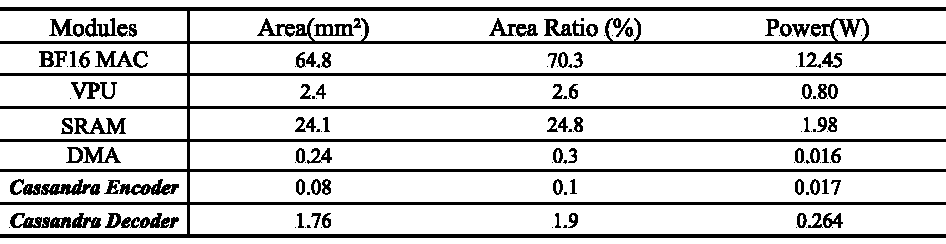
\includegraphics[width=\colimgwidth]{Tables/6_4_Power_and_Area.pdf}
\label{table_6_4}
\vspace{-0.20in}
\end{table}



